\chap{Cardiovascular Magnetic Resonance Imaging}
The intent of this chapter is to give a brief overview of the history of cardiovascular magnetic resonance (CMR) \Nomenclature{CMR}{Cardiovascular magnetic resonance} imaging and to discuss emerging methods, in particular with respect to self-gated and non-Cartesian methods. 

\sect{A brief overview}
The earliest recorded use of magnetic resonance for probing the function of the heart was Phosphorus-31 NMR spectroscopy of tissue metabolites in ischemic rat hearts~\cite{Hoult1974,Gadian1976,Jacobus1977}. Functional imaging of the heart was introduced with the advent of so-called cine imaging~\cite{Herfkens1983,Lanzer1984,Waterton1985,Sechtem1987a} where the image acquisition was gated using an external electrocardiogram (ECG) \Nomenclature{ECG}{Electrocardiogram} signal. The development of cine methods has enabled accurate measurements of ventricular volumes~\cite{Sechtem1987b} and ejection fractions~\cite{Utz1987}, which are essential functional parameters for determining and diagnosing heart failure. Initial developments in cine imaging used prospective gating and continuous acquisition of one k-space line per heartbeat. This allowed for a very high temporal resolution, but it meant that the acquisition time had to be adapted to the shortest RR-interval. In order not to run into the next heartbeat, the last part of diastole was discarded. With the introduction of the FASTCARD method~\cite{Foo1995}, several lines were acquired repeatedly during the same heartbeat. Using retrospective sorting of the images, it was then possible to cover the entire cardiac cycle, even though there were variations in RR-intervals~\cite{Lenz1989}. To further improve the precision, non-linear stretching of the cardiac cycle has been proposed based on empirical observations of the duration of systole and diastole, respectively~\cite{Feinstein1997}. The continued improvement of the cine imaging techniques means that CMR has developed into a highly accurate method for quantification of cardiac function~\cite{VanDerGeest1999}, and is now considered the non-invasive reference standard~\cite{Pennell2004} for quantifying ventricular volumes, ejection fraction and myocardial mass~\cite{Kramer2020}.

\sect{Free breathing}
The inherent motion sensitivity of cardiac MRI will often require the patient to hold their breath. The heart is resting directly on top of the diaphragm, meaning that breathing motion will change the position of the heart, resulting in motion artifacts. A clinical CMR exam will typically require the patient to hold their breath repeatedly and for extended periods. This precludes the very sickest populations, as cardiovascular disease is often associated with dyspnea. Because of this, it is desirable to acquire images during free breathing.

The earliest example of free-breathing cardiac MRI in the literature refers to measurements of cardiac output in mice, where free-breathing imaging was compared to controlled mechanical ventilation~\cite{Whalen1991}. Prospective navigator gating has been suggested as a viable method for free-breathing coronary angiography~\cite{Danias1997}. By placing exciting a spatially-selective excitation~\cite{Pauly1989} over the liver dome~\cite{McConnell1997}, the acquisition could be triggered or gated according to the respiratory position. An alternative method is to use an external pressure-sensing bellow that can be strapped to the chest or abdomen of the patient to detect respiration, that then can be used similar to a navigator~\cite{Santelli2011}. A potential drawback of using a respiratory bellow is the inherent phase shift between the diaphragmatic position and the abdominal height~\cite{Pengelly1979}. An example of this phase shift can be observed in Figure~\ref{fig:pca_resp}.

\sect{Self-gating}
Conventionally, cine imaging will require an external signal, such as an ECG-signal from the patient ECG to gate or trigger the signal. By a broader definition, a navigator could also be considered an external signal, as it requires setup and planning separate from the imaging sequence. The purpose of self-gating is to derive one or several of these external signals from the data itself~\cite{Larson2004}. As the ECG is typically required for many of the imaging sequences, the most common method has been to use respiratory self-gating to enable free-breathing~\cite{Larson2005}, but methods combining cardiac and respiratory self-gating have also been suggested~\cite{Larson2003:RSNA, DiSopra2019}.

Methods for self-gating can mostly be divided into methods based on image metrics~\cite{McGee2000,Manduca2000}, or methods deriving the motion signal from the raw k-space. Methods that derive motion from k-space usually consider the k-space center signal~\cite{Buehrer2008}, but it is also common to use a single k-space line as an image projection from which motion can be derived~\cite{Pang2014}. Image-based self-gating is often based on reconstructing a real-time image series\cite{Riederer1988, Nayak2004}, from which motion can be estimated, either by simply registering images together~\cite{Kellman2009, Hansen2012, Xue2013}, or by placing an ROI where respiratory or cardiac motion can be observed, such as on the interface between the liver dome and the lung, or in the myocardium of the heart~\cite{Paul2015}.

\begin{figure}
    \centering
    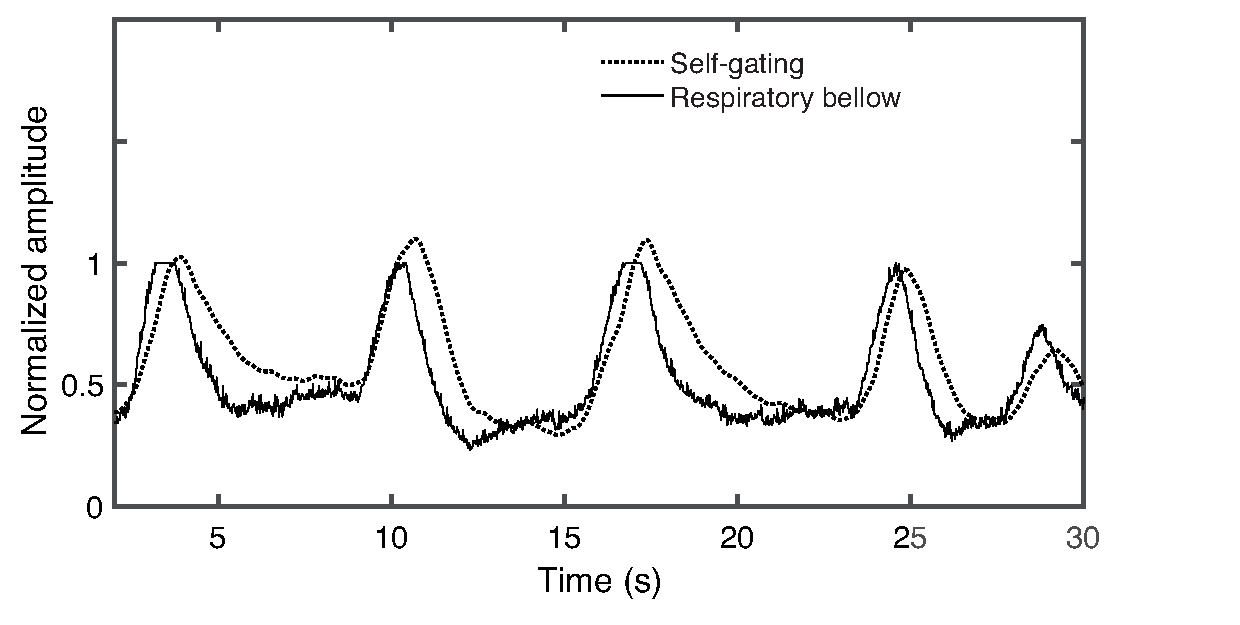
\includegraphics[width=0.75\textwidth]{pca_resp}
    \caption{An example of respiratory motion as detected by a respiratory bellow strapped the patient's abdomen, to record pressure changes due to respiration (solid line). Overlaid is a self-gating signal calculated using principal component analysis of the k-space center (dashed line). }
    \label{fig:pca_resp}
\end{figure}

\begin{figure}
    \centering
    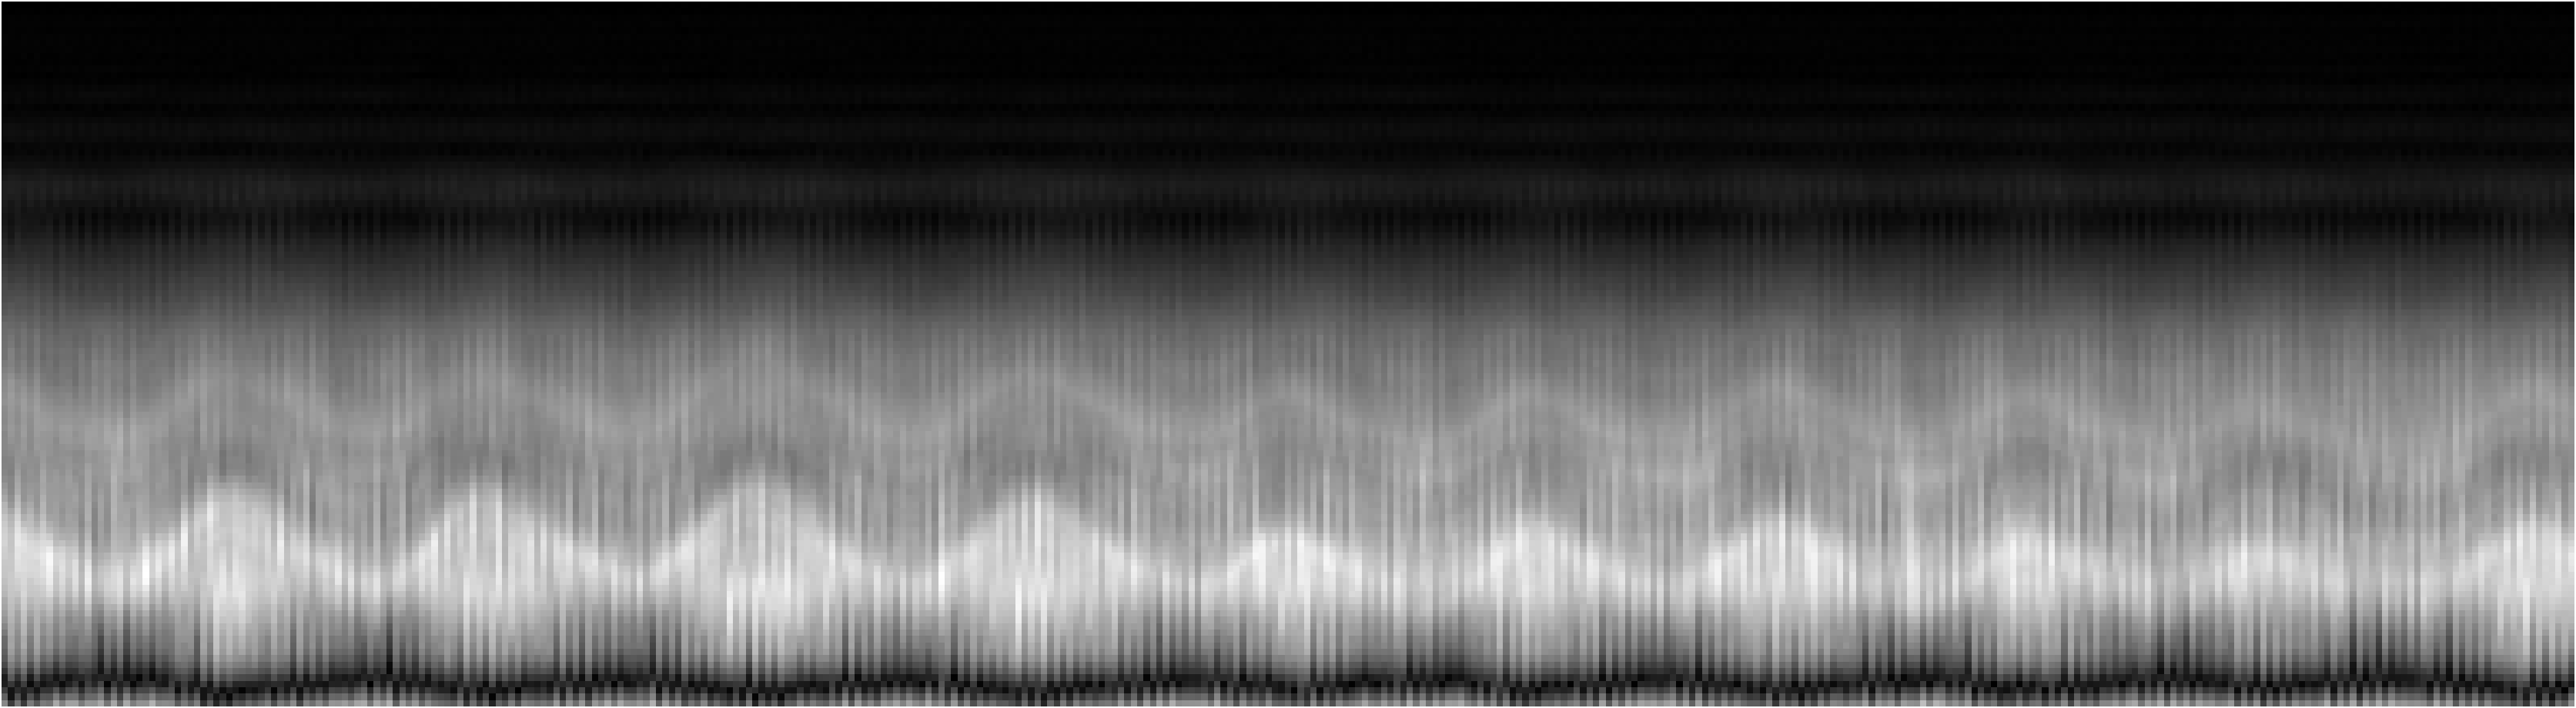
\includegraphics[width=\textwidth]{proj_nav.png}
    \caption{An example of respiratory motion as detected by a projection navigator. }
    \label{fig:proj_resp}
\end{figure}

An example of projection-based self-gating has been combined with the golden-angle by interleaving the readout with a spoke measured in the same direction, with a suitable frequency. This can be done both in 2D~\cite{Kramer2014} and 3D~\cite{Pang2014}.

%\sect{Tissue phase-mapping}
%In a previous section, the phase-contrast method was discussed in the context of measuring flow. However, phase contrast is not limited to flow measurements, and can also be used for tissue velocity measurements~\cite{Paelinck2005}. Tissue velocities are routinely used in Doppler echocardiography as a surrogate measure of left ventricular filling pressures and is a key factor in assessing Diastolic function together with transmitral blood flow velocities~\cite{Silbiger2019}. Tissue-phase contrast have previously been combined with the golden-angle profile ordering~\cite{Paul2016} with image-based self-navigation~\cite{Paul2016b}.